\chapter{Data Appendix}
\label{sec:Appendix}

\begin{figure}[H]
\centering
Estimated CAFTA-DR tariffs computed using the following scheme:
\begin{tabular}{lll}
\hline Cat. & Number & Phase Out Scheme \\
& of Goods & \\
\hline
A &4326&Good is now duty free (0\% tariff rate).\\
B & 381&Good will be reduced to duty free in 5 equal annual stages, duty free by 2012.\\
C & 692&Good will be reduced to duty free in 10 equal annual stages, duty free by 2017.\\
D & 121&Good will be reduced to duty free in 15 equal annual stages, duty free by 2022.\\
G & 903&Good remains duty free.\\
M & 313& 2007-2008 reduced by 2\% of base rate. 2009-2013 reduced by 8\% of base rate. \\
& & 2014-2016 reduced by 16\% percent of base rate. Duty free by 2017.\\
N & 22 & Good will have tariff rate reduced in 12 equal annual stages, duty free by 2019.\\
SP& 48 & Special exemption, usually means good has a non-tariff barrier such as a quota.\\
V &  2 & Good will remain at base rate until 2017. From 2017-2022 reduced by 8\% of\\
& & base rate, 2022-2026 reduced by 12 percent of base rate. Duty free by 2027.\\
W &  2 & Good will have tariff rate reduced in 4 equal annual stages, duty free by 2011.\\
X & 21 & Good will have tariff rate reduced in 4 equal annual stages (first year is exempt),\\ 
& & duty free by 2012. \\
Y & 2  & Good will have duties reduced by 15 percent of base rate for first five years\\
& & (2007-2012), 5\% for next four years after that (2012-2016), duty free by 2017.\\
\end{tabular}
\caption{\label{fig:Appendix1}}
Source: \citet{ustraderep}, CAFTA-DR Annex 3.3
\end{figure}

\begin{figure}[H]
\centering
Conversion Table for DHS occupations to ISIC 2 digit code
\scriptsize
\begin{tabular}{ll}
Occupation & ISIC 2 digit\\ \hline
peones de la industria manufacturera & 15,16,17,18,19,20,21,22,23,24,25\\
&26,27,28,29,30,31,32,33,34,35,36,37\\
conductores de veh\'{i}culos de motor & 60\\
personal de enfermer\'{i}a y parter\'{i}a de nivel superior & 85\\
profesionales de nivel medio de servicios de administraci\'{o}n & 74\\
m\'{e}dicos y profesionales afines (excepto el personal de enfermer\'{i}a y parter\'{i}a) & 85,86\\
vendedores y demostradores de tiendas y almacenes & 52\\
maestros de nivel superior de la ense\~{n}anza primaria y preescolar & 80\\
vendedores de quioscos y de puestos de mercado & 52\\
personal dom\'{e}stico y afines, limpiadores, lavanderos y planchadores & 90\\
profesionales en ciencias biol\'{o}gicas y otras disciplinas relativas a los seres o & 73\\
otros directores de departamentos & 74\\
oficiales y operarios de la construcci\'{o}n (obra gruesa) y afines & 45\\
peones de la miner\'{i}a y la construcci\'{o}n & 10,11,12,13,14\\
agricultores y trabajadores calificados de cultivos para el mercado & 1\\
secretarios y operadores de m\'{a}quinas de oficina & 74\\
conserjes, lavadores de ventanas y afines & 90\\
mec\'{a}nicos y ajustadores de m\'{a}quinas & 50\\
mec\'{a}nicos y ajustadores de equipos el\'{e}ctricos y electr\'{o}nicos & 40\\
mensajeros, porteadores, porteros y afines & 53,93\\
otros profesionales de la ense\~{n}anza & 80\\
otros trabajadores de servicios personales a particulares & 93\\
oficiales y operarios del tratamiento de la madera, ebanistas y afines & 20,36\\
peones del transporte & 63\\
personal de los servicios de protecci\'{o}n y seguridad & 75\\
productores y trabajadores agropecuarios calificados% cuya producci\'{o}n se destina 
& 1\\
t\'{e}cnicos en programaci\'{o}n y control inform\'{a}ticos & 72\\
profesionales de nivel medio en operaciones financieras y comerciales & 65\\
oficiales y operarios de los textiles y de la confecci\'{o}n y afines & 17,18\\
oficiales y operarios de la construcci\'{o}n (trabajos de acabado) y afines & 45\\
cajeros, taquilleros y afines & 65\\
maestros de nivel medio de la ense\~{n}anza primaria & 80\\
trabajadores de los cuidados personales y afines & 93\\
don't know & 99\\
peones agropecuarios, forestales, pesqueros y afines & 01,05\\
operadores de equipos \'{o}pticos y electr\'{o}nicos & 72,33\\
vendedores ambulantes y afines & 52\\
gerentes de empresa & 74\\
personal de intendencia y de restauraci\'{o}n & 55\\
empleados encargados del registro de materiales y de transportes & 60,63\\
herreros, herramentistas y afines & 28,29 \\
miembros del poder ejecutivo y de los cuerpos legislativos & 75\\
directores de departamentos de producci\'{o}n y operaciones & 74\\
t\'{e}cnicos en ciencias f\'{i}sicas y qu\'{i}micas y en ingenier\'{i}a & 74,24\\
operadores de instalaciones de vidrier\'{i}a, cer\'{a}mica y afines & 26\\
fuerzas armadas & 75\\
pescadores, cazadores y tramperos & 1,5\\
arquitectos, ingenieros y afines & 74\\
empleados de servicios de informaci\'{o}n a la clientela & 64,72\\
pintores, limpiadores de fachadas y afines & 45,91\\
moldeadores, soldadores, chapistas, caldereros%, montadores de estructuras met\'{a}li 
& 28,29,3\\
otros operadores de m\'{a}quinas y montadores & 15,16,17,18,19,20,21,22,23,24,25,26\\
&27,28,29,30,31,32,33,34,35,36,37
\end{tabular}
\caption{\label{fig:Appendix2}}
\end{figure}

\begin{figure}[H]
\centering
\scriptsize
\begin{tabular}{ll}
Occupation & ISIC 2 digit\\ \hline
operadores de m\'{a}quinas para fabricar productos textiles y art\'{i}culos de piel y cu & 17,19\\
personal directivo de la administraci\'{o}n p\'{u}blica & 75\\
personal al servicio directo de los pasajeros & 60\\
jefes de peque\~{n}as poblaciones & 75\\
inspectores de obras, seguridad y salud y control de calidad & 74 \\
profesionales de nivel medio de actividades art\'{i}sticas, espect\'{a}culos y deportes & 92\\
profesores de universidades y otros establecimientos de la ense\~{n}anza superior & 80 \\
operadores de instalaciones de procesamiento de la madera y de la fabricaci\'{o}n de & 20,21\\
oficiales y operarios del procesamiento de alimentos y afines & 15,16\\
criadores y trabajadores pecuarios calificados de la cr\'{i}a de animales para el me & 1\\
archiveros, bibliotecarios, documentalistas y afines & 92\\
otros oficinistas & 74\\
alfareros, operarios de cristaler\'{i}as y afines & 52\\
profesionales del derecho & 75\\
operadores de maquinaria agr\'{i}cola m\'{o}vil y de otras m\'{a}quinas m\'{o}viles & 1\\
sacerdotes de distintas religiones & 91\\
recolectores de basura y afines & 90\\
operadores de m\'{a}quinas para fabricar productos de caucho y de material pl\'{a}stico & 25\\
limpiabotas y otros trabajadores callejeros & 52,93\\
astr\'{o}logos, adivinadores y afines & 93\\
operadores de m\'{a}quinas para fabricar productos qu\'{i}micos & 24\\
operadores de m\'{a}quinas para elaborar alimentos y productos afines & 15\\
especialistas en ciencias sociales y humanas & 73\\
oficiales y operarios de las pieles, cuero y calzado & 18,19\\
operadores de m\'{a}quinas de imprenta, encuadernaci\'{o}n y fabricaci\'{o}n de productos de & 21,22\\
profesionales de nivel medio de la medicina moderna y la salud (excepto el perso & 85\\
operadores de m\'{a}quinas para trabajar metales y productos minerales & 26,27,28\\
otros maestros e instructores de nivel medio & 80\\
profesores de la ense\~{n}anza secundaria & 80\\
maestros de nivel medio de la ense\~{n}anza preescolar & 80\\
empleados de bibliotecas y servicios de correos y afines & 92\\
especialistas en organizaci\'{o}n y administaci\'{o}n de empresas  y afines & 74\\
oficiales y operarios de las artes gr\'{a}ficas y afines & 92\\
operadores de instalaciones mineras y de extracci\'{o}n y procesamiento de minerales & 10,11,12,13,14\\
operadores de instalaciones de producci\'{o}n de energ\'{i}a y afines & 40\\
trabajadores y asistentes sociales de nivel medio & 85\\
personal de enfermer\'{i}a y parter\'{i}a de nivel medio & 85\\
f\'{i}sicos, qu\'{i}micos y afines & 74,24\\
trabajadores forestales calificados y afines & 2\\
other & 99\\
agentes de las administraciones p\'{u}blicas de aduanas, impuestos y afines & 75\\
escritores, artistas creativos y ejecutantes & 92\\
montadores & 29,30,31,32,33,34,35,36\\
directores generales y gerentes generales de empresa & 74\\
agentes comerciales y corredores & 70\\
mec\'{a}nicos de precisi\'{o}n en metales y materiales similares & 26,27,28\\
profesionales de la inform\'{a}tica & 72\\
t\'{e}cnicos de nivel medio en ciencias biol\'{o}gicas, agronom\'{i}a, zootecnia y afines & 1\\
auxiliares laicos de los cultos & 91\\
marineros de cubierta y afines & 61\\
dirigentes y administradores de organizaciones especializadas & 74\\
t\'{e}cnicos en navegaci\'{o}n mar\'{i}tima y aeron\'{a}utica & 61,62\\
auxiliares contables y financieros & 74\\
modelos de modas, arte y publicidad & 92\\
maestros e instructores de nivel superior de la ense\~{n}anza especial & 80
\end{tabular}

\normalsize
Figure \ref{fig:Appendix2}
\end{figure}

\begin{landscape}
\begin{figure}[H]
\centering
Average hours worked per week for a given economic activity in 2002
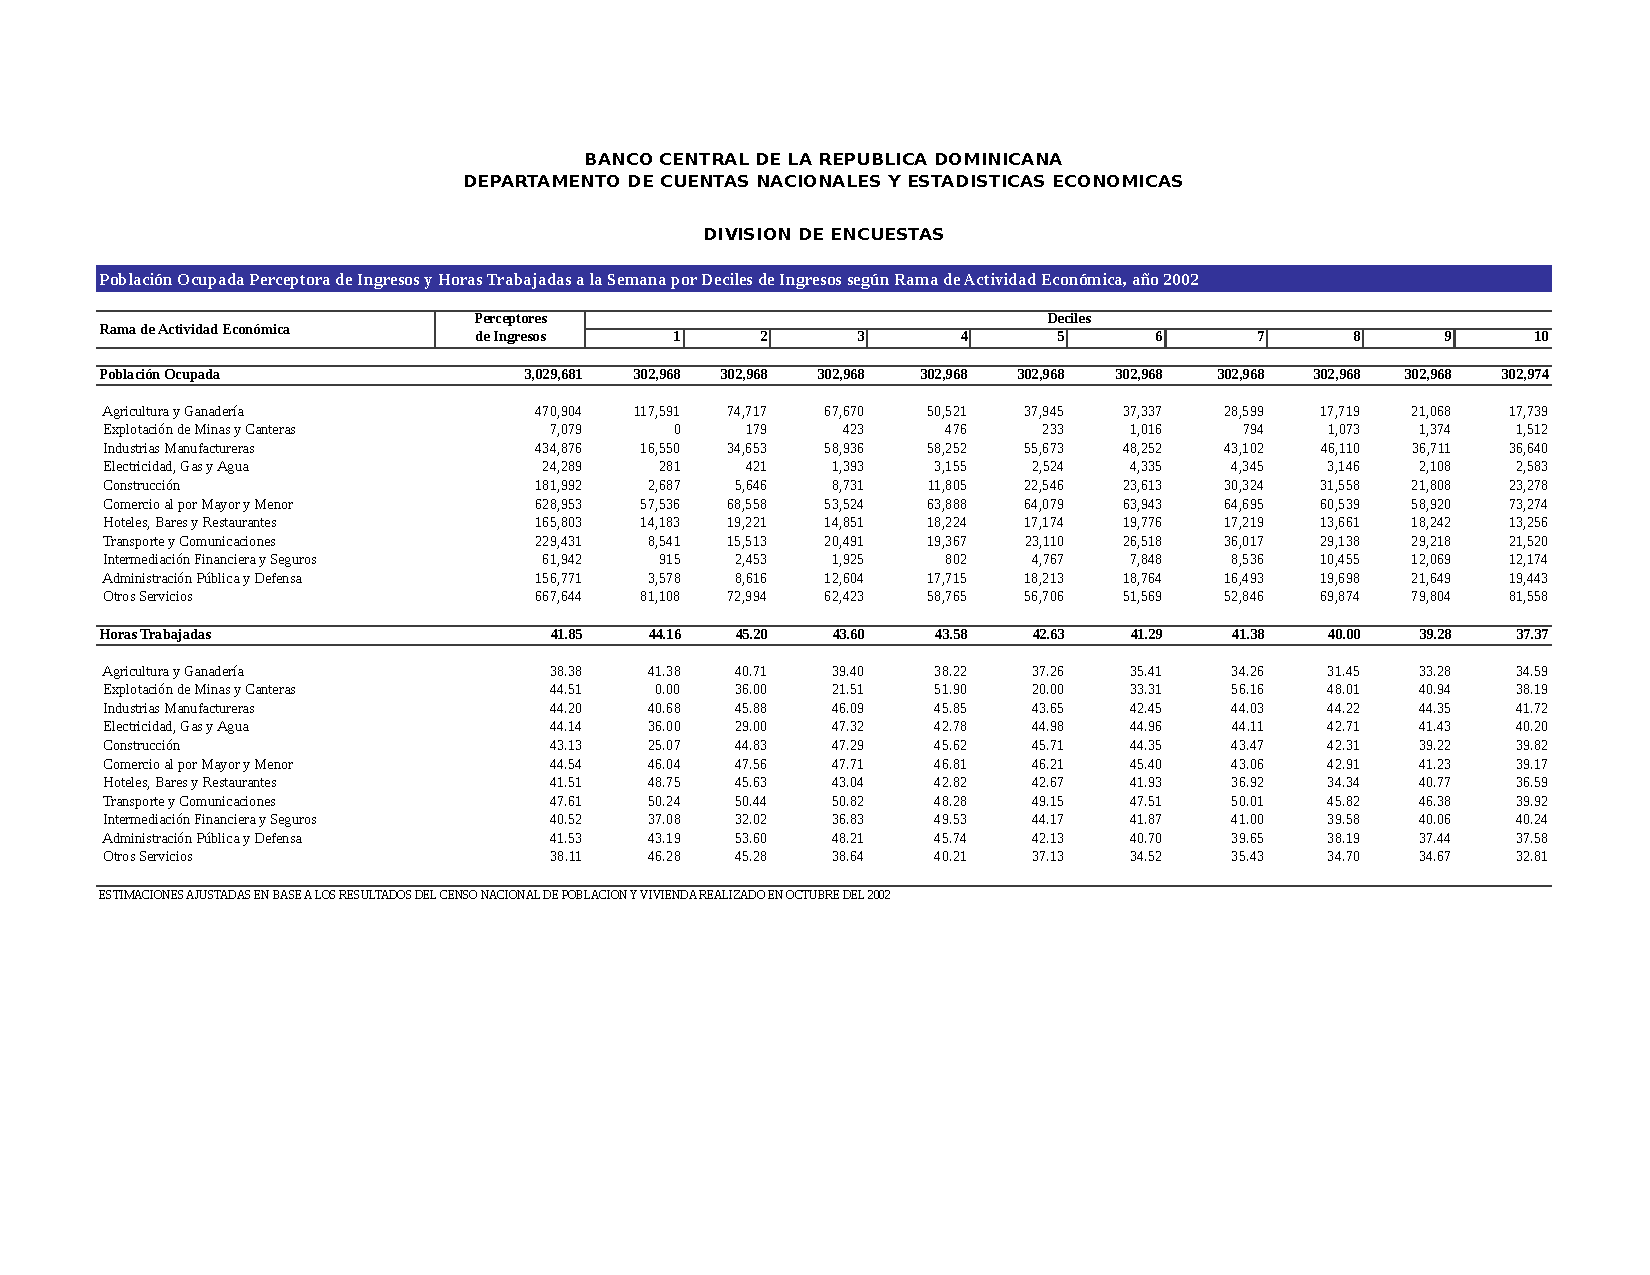
\includegraphics[width=\hsize,keepaspectratio=true]{../Plots/AvgHoursOcc2002.pdf}
\caption{\label{fig:Appendix3}}
Source: Central Bank of the Dominican Republic
\end{figure}
\end{landscape}

\begin{landscape}
\begin{figure}[H]
\centering
Average  hours worked per week for a given economic activity in 2013
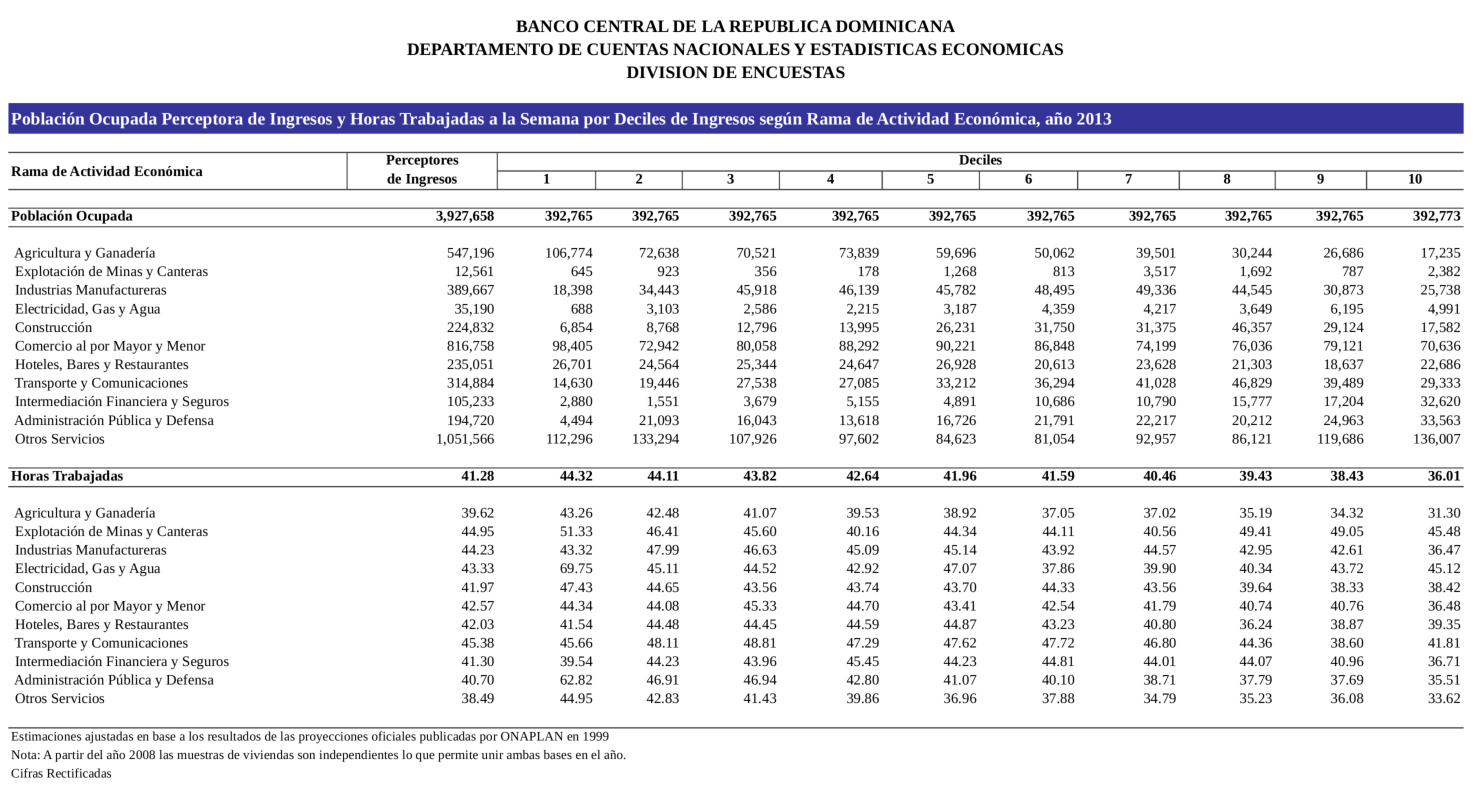
\includegraphics[width=\hsize,keepaspectratio=true]{../Plots/AvgHoursOcc2013.pdf}
\caption{\label{fig:Appendix4}}
Source: Central Bank of the Dominican Republic
\end{figure}
\end{landscape}